
\documentclass[a4paper, 11pt]{article}

%%%%%%%%%%%%%%%%%%%%%%%%%%%%%%
\oddsidemargin  0.0in
\evensidemargin 0.0in
\textwidth      6.2in
\headheight     0.0in
\topmargin      0.0in
\textheight=9.4in
\parindent=0in
%%%%%%%%%%%%%%%%%%%%%%%%%%%%%%


\usepackage{amsthm,amsfonts,amssymb,amsmath}
\usepackage[small,compact]{titlesec}

\usepackage[utf8]{inputenc} 

\usepackage[francais]{babel}

\usepackage{pdfpages}
\usepackage{multicol}
\usepackage{multirow}
\usepackage{array}
\usepackage{verbatim}


\newcommand{\esp}{\mathbb{E}}
\newcommand{\var}{\mathbb{V}\text{ar}}
\newcommand{\cov}{\mathbb{C}\text{ov}}
\newcommand{\corr}{\mathbb{C}\text{orr}}
\newcommand{\prob}{\mathbb{P}}
\newcommand{\N}{\mathcal{N}}
\def\I{\mathbb{I}}
\def\R{\mathbb{R}}
\def\P{{\mathbb P}}
\newcommand{\bm}{\boldmath}
\newcommand{\um}{\unboldmath}
\newcommand{\botheta}{\mbox{\bm$\theta$\um}}
\newcommand{\boTheta}{\mbox{\bm$\Theta$\um}}
\newcommand{\boY}{\mbox{\bm$Y$\um}}
\newcommand{\bobeta}{\mbox{$\boldsymbol\beta$}}
\newcommand{\boeps}{\mbox{\bm$\varepsilon$\um}}
\newcommand{\boldx}{\mbox{\bm$x$\um}}
\newcommand{\boR}{\mbox{\bm$R$\um}}
\newcommand{\boun}{\mbox{\bm$1$\um}}
\newcommand{\boz}{\mbox{\bm$0$\um}}
\newcommand{\bolambda}{\mbox{\bm$\lambda$\um}}
\newcommand{\bov}{\mbox{\bm$v$\um}}
\newcommand{\boalpha}{\mbox{\bm$\alpha$\um}}
\newcommand{\bo}[1]{\mbox{\bm$#1$\um}}
\newcommand{\boX}{\mbox{$\boldsymbol{X}$}}
\newcommand{\boV}{\bo{V}}
\newcommand{\hbobeta}{\widehat{\bobeta}}
\newcommand{\hboeps}{\widehat{\boeps}}
\newcommand{\hY}{\widehat{\boY}}
\newcommand{\boH}{\bo{H}}
\newcommand{\boI}{\bo{\I}}
\newcommand{\eproof}{\hfill$\sqcap\!\!\!\!\sqcup$}
\newcommand{\bou}{\mbox{\bm$u$\um}}


\usepackage{fancyhdr}
\pagestyle{fancy}

\renewcommand{\headrulewidth}{1pt}
%\fancyhead[C]{Automne 2023} 
%\fancyhead[L]{STT-2100 Régression}
%\fancyhead[R]{Julien Miron}
\fancyhead[C]{STT-2100 Régression}

\begin{document}
	
	\medskip
	\begin{center}
		{\Large Feuille de formules - Examen 2}
	\end{center}


\medskip
\underline{Régression linéaire multiple avec $p$ variables et des erreurs normales. ($p'=p+1$)} \\

\medskip\medskip
\begin{itemize}
	\item[$\bullet$] $\hbobeta=(\boX' \boX)^{-1} \boX' \boY$; \hspace{0.5 cm} $ \hbobeta \sim \mathcal{N}_p\{\bobeta,\; \sigma^2 (\boX'\boX)^{-1}\}$; \hspace{0.5 cm} $ \widehat{\sigma}^2 =\frac{\hboeps'\hboeps}{n-p'} $; \hspace{0.5 cm} $ \boH=\boX(\boX'\boX)^{-1}\boX'$

	\medskip\medskip\medskip\medskip
	\item[$\bullet$] Combinaison linéaire de $\bobeta$: $\theta = \boalpha' \bobeta $ 
	  $$ \widehat{\theta}  = \boalpha' \widehat{\bobeta} \; \sim \;  \N(\bo a'\bobeta, \; \sigma^2\bo a'(\boX'\boX)^{-1}\bo a) 
	  \quad\quad \text{et} \quad\quad
	  \frac{\bo a'\hbobeta-\theta}{\sqrt{\widehat{\sigma}^2\bo a'(\boX'\boX)^{-1}\bo a}} \; \sim \; \mathcal{T}_{n-p'}$$

	\medskip\medskip\medskip\medskip
	\item[$\bullet$] Intervalles de confiance: \medskip

$$\left[ \widehat\beta_i\pm t_{n-p',1-\alpha/2}\sqrt{\widehat{\sigma}^2 v_{ii}} \right], \; \; \mbox{ avec   } V = (\bo X' \bo X)^{-1} $$\medskip
$$ \left[\displaystyle\bo{x^*}'\hbobeta\pm t_{n-p', 1-\alpha/2}\sqrt{\widehat{\sigma}^2\bo{x^*}'(\boX'\boX)^{-1}\bo{x^*}}\right] \hspace{0.2 cm} ou \hspace{0.2 cm} \left[\bo{x^*}'\hbobeta\pm t_{n-p', 1-\alpha/2}\sqrt{\widehat{\sigma}^2\left(1+\bo{x^*}'(\boX'\boX)^{-1}\bo{x^*}\right)}\right]$$

	\medskip\medskip\medskip\medskip
	\item[$\bullet$] Test de $F$ global de la régression: \medskip
$$F={SC_{reg}/p\over SC_{res}/(n-p')}={SC_{reg}/p\over \widehat{\sigma}^2}= \frac{CM_{reg}}{CM_{res}}; \quad \mbox{ rejet de $H_0$ si } F > F_{p,n-p', 1-\alpha}$$
 
	\medskip\medskip\medskip\medskip
	\item[$\bullet$] Test de réduction de modèle: \medskip

\begin{equation*}\label{F:ESS}
F={SC_{res}^{(0)}-SC_{res}^{(1)}\over \Delta_{dl} \widehat{\sigma}^2_{H_1}}; \quad \mbox{ rejet de $H_0$ si  } F\ge F_{\Delta_{dl},n-p', 1-\alpha}
\end{equation*}

\medskip
où $SC_{res}^{(0)}$ = $SC_{res}$ du modèle réduit, $SC_{res}^{(1)}$ = $SC_{res}$ du modèle complet, 

\medskip
 $\Delta_{dl}=dl(SC_{res}^{(0)})-dl(SC_{res}^{(1)})$, et  $\widehat{\sigma}_{H_1}^2 = $ estimation de $\sigma^2$ avec le modèle complet. 

	\medskip\medskip\medskip\medskip
	\item[$\bullet$] Test d'une hypothèse linéaire générale: $H_0:~\bo{C}\bobeta=\bo{d}$ vs $H_1:~\bo{C}\bobeta \neq \bo{d}$
	
	\medskip
$$F={ (\bo{C}\hbobeta-\bo{d})'[\bo{C}(\boX'\boX)^{-1}\bo{C}']^{-1}(\bo{C}\hbobeta-\bo{d})\over r \widehat{\sigma}^2_{H_1}} \sim F_{r, n-p'}$$

\medskip
où $r$ est le nombre nombre de lignes de la matrice $C$.\\


\newpage

	\item[$\bullet$] Critères de comparaison de modèles:
	
	\begin{center}
		\begin{tabular}{ll}
     $\displaystyle R^2={SC_{reg}\over SC_{tot}}=1-{SC_{res}\over SC_{tot}}$
     & $\displaystyle R^2_{a}=1-{CM_{res}\over CM_{tot}}=1-{SC_{res}/(n-p')\over SC_{tot}/(n-1)}$\medskip\\\medskip
     
      $\displaystyle \mbox{BIC}=n\ln(SC_{res}/n)+ p \log(n)$
     & $\displaystyle \mbox{AIC}=n\ln(SC_{res}/n)+2p'.$\\ 
     PRESS = $\displaystyle \sum_{i=1}^n (\widehat{\varepsilon}_{i,-i})^2 = \sum_{i=1}^n\left({\widehat\varepsilon_i\over1-h_{ii}}\right)^2$
     & $\displaystyle  C_p = p' + \frac{(\widehat{\sigma}_p^2-\widehat{\sigma}_{toutes}^2)(n-p')}{\widehat{\sigma}_{toutes}^2} $ \medskip\\\medskip
    
	    $ \displaystyle R^2_{p}=1- \frac{PRESS}{SC_{tot}} = 1 - \frac{\sum\limits_{i=1}^n(Y_i-\widehat{Y}_{i,-i})^2}{\sum\limits_{i=1}^n(Y_i-\bar{Y})^2} $  &
\end{tabular}
\end{center}





\item[$\bullet$] Diagnostiques:

\begin{center}
\begin{tabular}{l|l}
Diagnostique & Valeurs problématiques \\ \hline \\
$\displaystyle\mbox{VIF}_j= \frac{1}{1-R_j^2}$  & VIF $> 10 $ \\[6pt]
$\displaystyle\eta_j=\sqrt{\frac{\lambda_{max}}{\lambda_j}}$ & $\eta_j > 30$ \\[6pt]
$h_{ii}$ & $h_{ii} > 2p'/n$\\[6pt]
$\displaystyle T_i={\widehat\varepsilon_i\over \widehat{\sigma}_{-i}\sqrt{1-h_{ii}}} \sim\mathcal{T}_{n-p-2}$ & $|T_i|>2$ ou $|T_i|>t_{n-p-1, 1-\alpha^*/2}$, o\`u $\alpha^*=\alpha/n$ \\[6pt]
$\displaystyle DFFIT_i={\widehat{Y}_i-\widehat{Y}_{i,-i}\over \widehat{\sigma}_{-i}\sqrt{h_{ii}}}=T_i\sqrt{\frac{h_{ii}}{1-h_{ii}}}$ & $|DFFIT_i|>2$  ou $|DFFIT_i|>2\sqrt{p'/n}$ \\[6pt]
$\displaystyle DFFBETAS_{ji}={\widehat{\beta}_j-\widehat{\beta}_{j,-i}\over \widehat{\sigma}_{-i}\sqrt{(X'X)^{-1}_{jj}}}$ & $|DFBETA_{ji}|>2$  ou $|DFBETA_{ji} > 2 / \sqrt{n}$\\[6pt]
$\displaystyle C_i = {(\widehat{\bobeta}-\widehat{\bobeta}_{-i})'(\boX'\boX)(\widehat{\bobeta}-\widehat{\bobeta}_{-i}) \over p' \widehat\sigma^2}=\frac{\widehat{\varepsilon}_i^2h_{ii}}{(1-h_{ii})p'\widehat{\sigma}^2}$ & $C_i > 4 / (n-p')$ \\
$\displaystyle COVRATIO_i = {||Var(\widehat{\bobeta}_{-i})||\over||Var(\widehat{\bobeta})||||}$ & $\big|COVRATIO-1\big|>3p'/n$ 
\end{tabular}
\end{center}


Note : On peut ré-écrire $\displaystyle\widehat{\sigma}_{-i}=\sqrt{{(n-p)\widehat{\sigma}^2-\widehat\varepsilon_i^2/(1-h_{ii})\over n-p'}}$.


\medskip\medskip\medskip
\item[$\bullet$]  Régularisation:

\medskip
Régression ridge: On minimise $\displaystyle Q(\beta) = \sum_{i=1}^n (Y_i - X_i' \bobeta)^2 + \lambda \sum_{j=1}^p \beta_j^2 $.

\hspace{3cm} On obtient $\displaystyle\hbobeta(\lambda) = \{\boI+\lambda(\boX'\boX)^{-1}\}^{-1}\hbobeta$.


LASSO: On minimise  $\displaystyle Q(\beta) = \sum_{i=1}^n (Y_i - X_i' \bobeta)^2 + \lambda \sum_{i=1}^p | \beta_j | $.


\end{itemize}



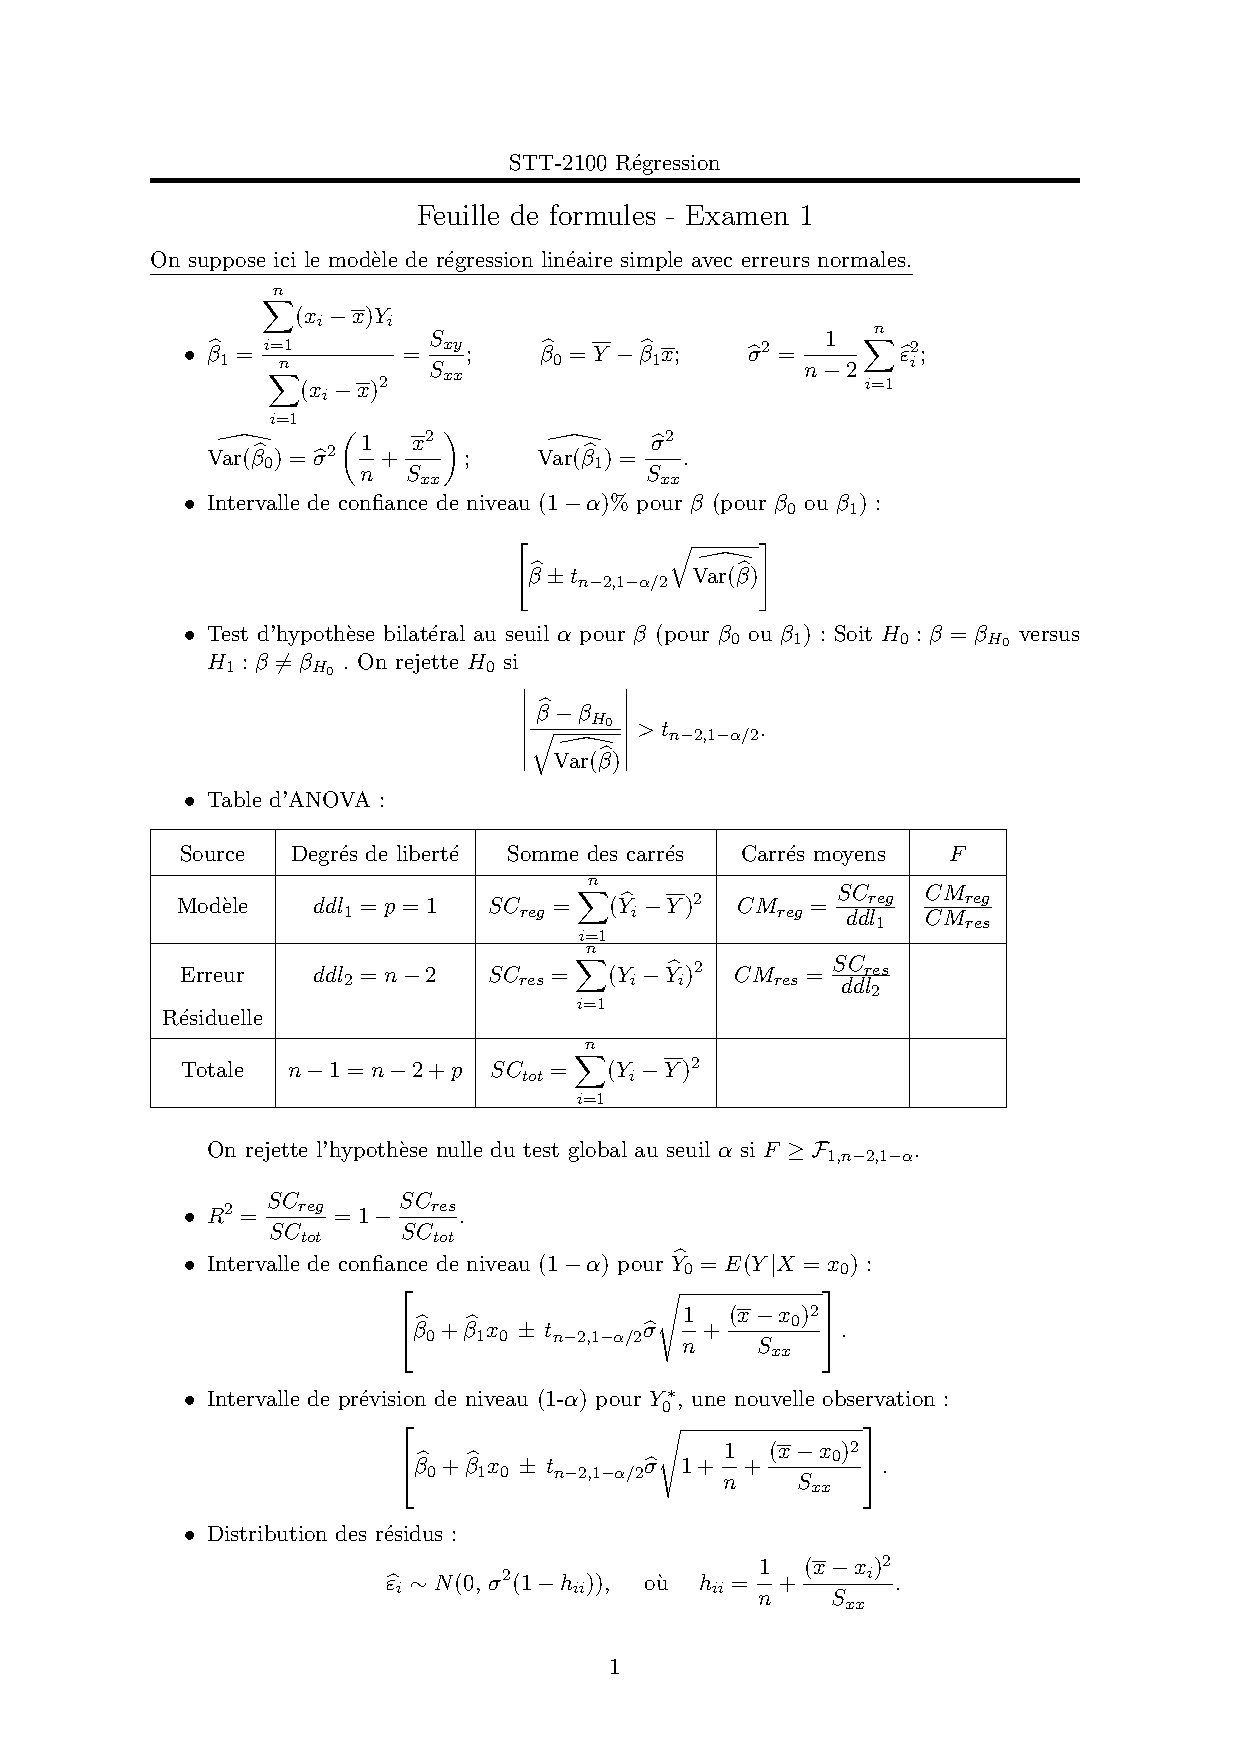
\includepdf{STT-2100-Formules-Examen1.pdf}

\end{document}
